\documentclass{article}
\usepackage{graphicx} 
\usepackage{wrapfig}
\usepackage{filecontents}
\usepackage{siunitx}
\usepackage[table]{xcolor}
\usepackage{float}
\usepackage{hyperref}

\usepackage{color} % balíček pro obarvování textů
\usepackage{xcolor}  % zapne možnost používání barev, mj. pro \definecolor
\usepackage{pgfplots} % http://www.chiark.greenend.org.uk/doc/texlive-doc/latex/pgfplots/pgfplots.pdf

\usepackage{multirow}
\usepackage{caption}

\captionsetup[figure]{labelformat=empty}


\ifnum 0\ifxetex 1\fi\ifluatex 1\fi=0 % if pdftex
  \usepackage[T1]{fontenc}
  \usepackage[utf8]{inputenc}
\else % if luatex or xelatex
  \ifxetex
    \usepackage{mathspec}
  \else
    \usepackage{fontspec}
  \fi
  \defaultfontfeatures{Ligatures=TeX,Scale=MatchLowercase}
\fi
\usepackage[total={175mm,230mm}, top=23mm, left=20mm, includefoot]{geometry}
\hypersetup{
    colorlinks,
    linkcolor={blue!50!black},
    citecolor={green!50!black},
    urlcolor={blue!80!black}
}
% \definecolor{fialova}{RGB}{ 255, 000, 255}
\definecolor{color-si1}{RGB}{ 255, 000, 000}
\definecolor{color-si2}{RGB}{ 251, 130, 032}

\definecolor{color-ge1}{RGB}{ 000, 255, 000}
\definecolor{color-ge2}{RGB}{ 032, 251, 160}

\definecolor{color-inp1}{RGB}{ 000, 000, 255}
\definecolor{color-inp2}{RGB}{ 160, 032, 251}

\definecolor{color-geas1}{RGB}{ 225, 225, 000}
\definecolor{color-geas2}{RGB}{ 225, 225, 100}

\definecolor{sedak}{RGB}{ 100, 100, 100}


\newcommand \obr[1]
{ obr.~\ref{#1}}

\newcommand \tab[1]
{ tab.~ß\ref{#1}}


\begin{document}

\section*{Zpracujte přehled připojovacích technologií pro metalické vodiče s uvedením výhod a nevýhod jednotlivých postupů}

Vypracoval: Tomáš Vavrinec - 240893

\section{Připojování vodičů bez odizolování}

\subsection{Typy připojování - spoje}
\begin{itemize}
  \item Rozebíratelné
  \item Nerozebíratelné
\end{itemize}

\begin{itemize}
  \item Šroubové
  \item Bezšroubové
\end{itemize}

\begin{itemize}
  \item S odizolováním
  \item Bez odizolování
\end{itemize}

\subsection{Šroubové systémy}
\begin{figure}[H]
  \begin{minipage}[r]{0.55\textwidth}
    \vspace{-15mm}
    Rozebíratelné spoje s odizolováním.
    Často pro připojení přívodních vodičů se síťovým napětím.
    Ve šroubu i ve vodiči vzniká pružná deformace.
    Spoj nesmí být po vytažení porušen. 
    Výhody:
    \begin{itemize}
      \item rozebiratelnost
      \item spolehlivé
    \end{itemize}
    nevýhody
    \begin{itemize}
      \item Potřeba nářadí (šroubovák/klíč)
    \end{itemize}
  \end{minipage}
  \hfil
  \begin{minipage}[r]{0.4\textwidth}
    \vspace{-15mm}
    \centering
    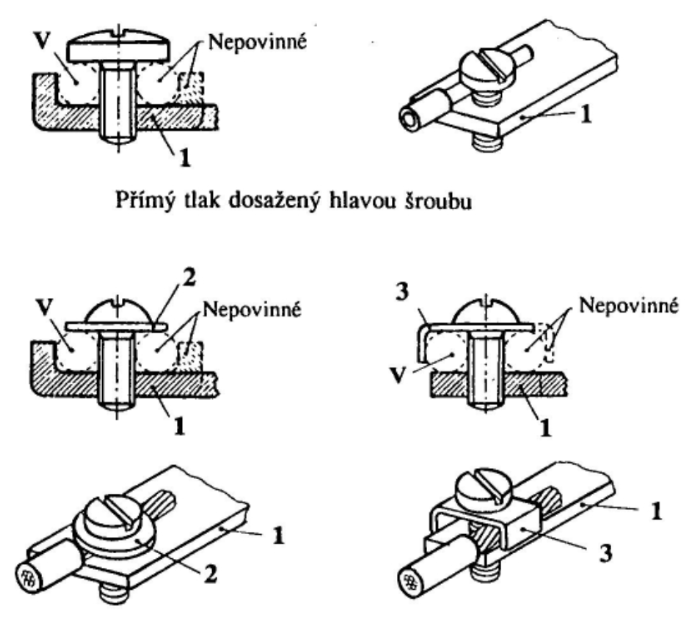
\includegraphics[width=\textwidth]{sroubovatko3.png}
    \caption{Hlavičkové šroubové spoje}
    % \label{fig:m-sch-sc-p6}
  \end{minipage}
\end{figure}

\begin{figure}[H]
  \begin{minipage}[t]{0.45\textwidth}
    \centering
    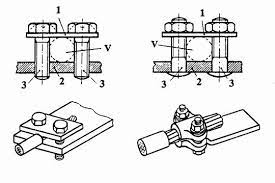
\includegraphics[width=\textwidth]{sroubovatko1.jpg}
    \caption{Příložkové šroubové spoje}
    % \label{fig:m-sch-sc-p6}
  \end{minipage}
  \hfil
  \begin{minipage}[t]{0.54\textwidth}
    \centering
    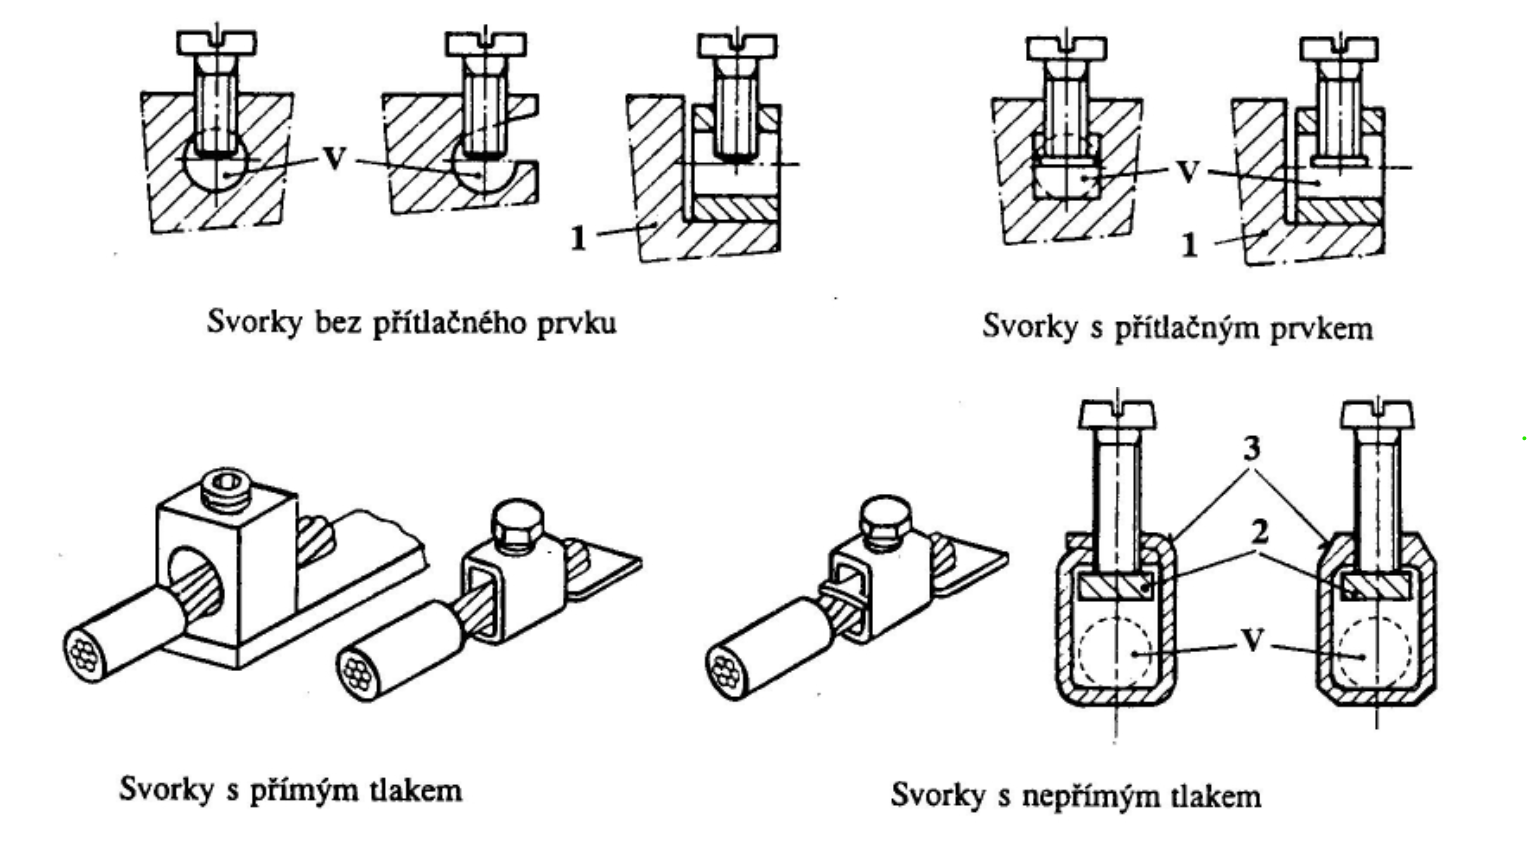
\includegraphics[width=\textwidth]{sroubovatko2.png}
    \caption{Zdířkové svorky}
    % \label{fig:m-sch-sc-p6}
  \end{minipage}
\end{figure}


% ---------------------------------------------------------------------------------
\subsection{Bezšroubové systémy}
Spoje s odizolováním. 
Často speciální nástroj k zasunutí a vysunutí vodiče.
\subsubsection{Nasouvací svorky (WAGO svorky)}
\begin{itemize}
  \item Stálý kontakt - přítlak pružinou
  \item Vzájemné spojení 2 a více vodičů
  \item Rozpojitelný systém - kónická svorka
  \item Výhody
  \begin{itemize}
    \item Rychlé a snadné používání
    \item Bez potřeby nářadí
    \item Spolehlivost
    \item Malé prostorové nároky
    \item Přehlednost 
  \end{itemize} 
  \item	Nevýhody
  \begin{itemize}
    \item Neuniverzálnost - speciální svorka pro různé průřezy vodičů
  \end{itemize}
\end{itemize}

\begin{figure}[H]
  \begin{minipage}[t]{0.35\textwidth}
    \centering
    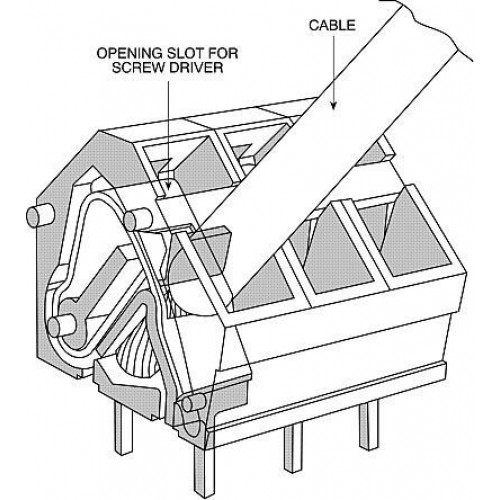
\includegraphics[width=\textwidth]{vagoSvorka2.jpg}
  \end{minipage}
  \hfil
  \begin{minipage}[t]{0.65\textwidth}
    \centering
    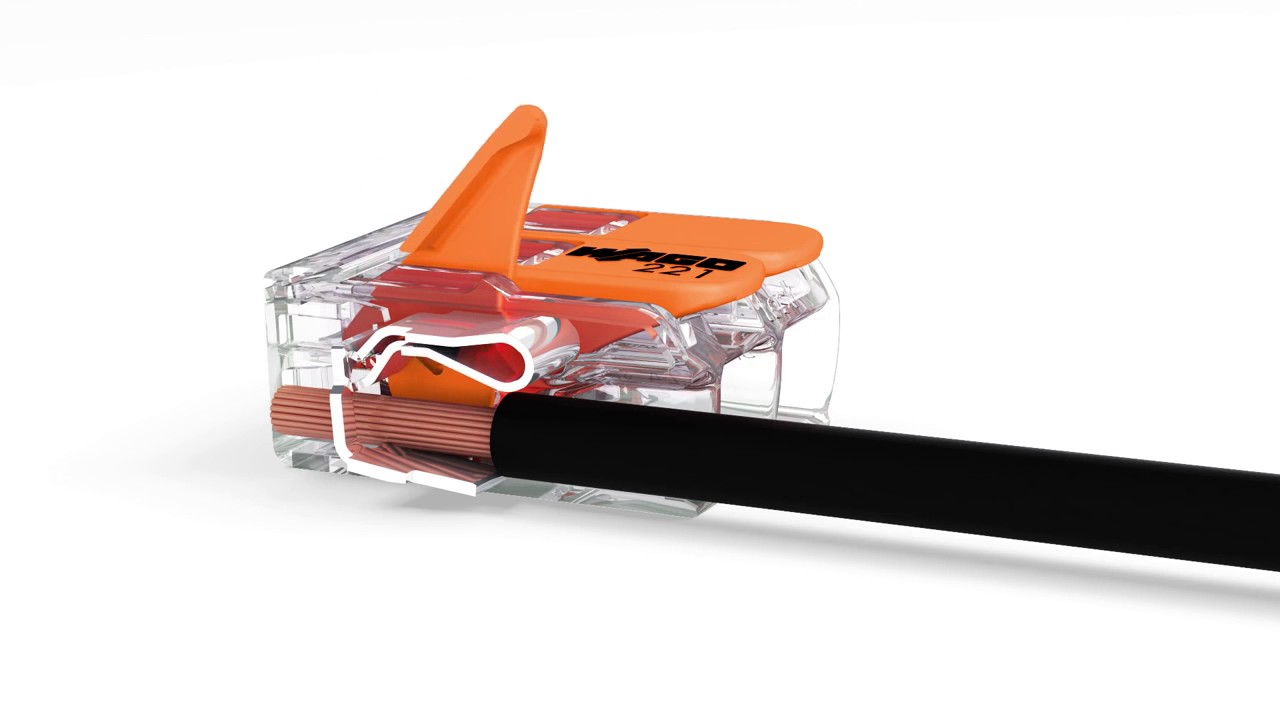
\includegraphics[width=\textwidth]{vagoSvorka1.jpg}
  \end{minipage}
  \caption{Nasouvací/pružinové svorky (WAGO svorky)}
\end{figure}

\newpage
\subsection{Pájené spoje}
\begin{itemize}
  \item Spojování pomocí roztaveného materiálu, tzv. pájkou, která má nižší teplotu tavení než spojované materiály.
  \item Nevýhody
  \begin{itemize}
    \item Nerozebíratelný spoj
    \item Je zapotřebí zvláštního nářadí
    \item Zdlouhavý technologicky náročný postup
    \item Nedosahují pevnosti svařovaných spojů
  \end{itemize}
  \item Výhody
  \begin{itemize}
    \item Lze spojit i nesvařitelné spoje (různé chemické složení spojovaných kovů)
    \item Nízká teplota pájení oproti svařování
    \item Pájka nepodléhá korozi
    \item Čistý proces
  \end{itemize}  
\end{itemize}

\begin{figure}[H]
  \begin{minipage}[t]{\textwidth}
    \centering
    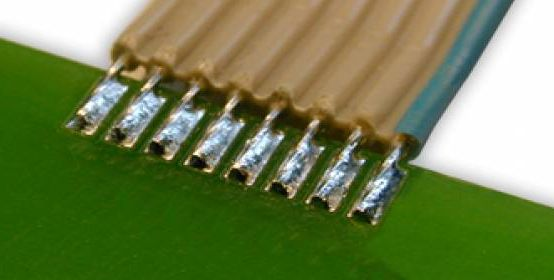
\includegraphics[width=\textwidth]{pajeni1.jpg}
    \caption{Pájený spoj}
    % \label{fig:m-sch-sc-p6}
  \end{minipage}
\end{figure}

\newpage
\subsection{Ovíjené spoje}

\begin{figure}[H]
  \begin{minipage}[t]{0.58\textwidth}
    \begin{itemize}
      \item Spojení mezi ovíjecím vodičem a ovíjeným trnem
      \item Záleží na výběru vodičů a nástrojů.
      \item Důležité je dodržení základních technologických kroků.
      \item Postupy - ruční, poloautomatický, automatický
      \item Nároky na vodiče
      \begin{itemize}
        \item Stejný odpor
        \item Mechanická pevnost - odolání namáhání při ovíjení
      \end{itemize}
      \item Typy spojů
      \begin{itemize}
        \item Pravé
        \item Modifikované
        \begin{itemize}
          \item První závit je ovinut s izolací
          \item Větší odolnost proti mechanickému namáhání - otřesy, vibrace, rázy
        \end{itemize}
      \end{itemize}
      \item	Výhody
      \begin{itemize}
        \item Opakovatelné a snadno rozebíratelné spoje
        \item Bez studených spojů
        \item Delší životnost než u pájených spojů
        \item Nevzniká teplo, které by poškozovalo součástky
        \item Nedochází k prasklinám a odlamování
        \item Čistota pracovního prostředí
        \item Vysoký tlak - docíleno bodového svařování za studena - plynotěsnost
      \end{itemize}
      \item Nevýhody
      \begin{itemize}
        \item Složitý proces
        \item Potřeba speciálního nářadí
        \item Nemožnost rychlé sériové výroby
        \item Větší spotřeba vodičů
        \item Po odvinutí se musí použít nový vodič
        \item Spoje musí být daleko od sebe (kvůli přístupu nástroje - ovíjecí pistole)
      \end{itemize}
    \end{itemize}    
  \end{minipage}
  \hfil
  \begin{minipage}[t]{0.4\textwidth}
    \begin{figure}[H]
      \centering
      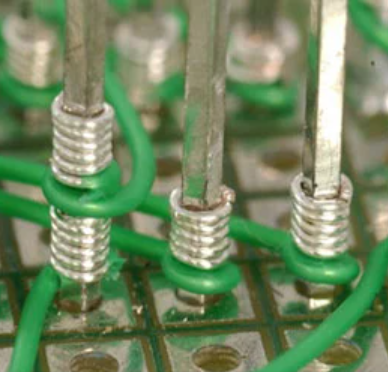
\includegraphics[width=\textwidth]{ovijen1.png}
      \caption{Ovíjený spoj}
    \end{figure}

    \begin{figure}[H]
      \centering
      
\includegraphics[width=\textwidth]{ovijen2.png}
      \caption{Ovíjený spoj}
    \end{figure}
  \end{minipage}
\end{figure}

\subsection{Systém TERMI-POINT}
\begin{itemize}
  \item Výhody
  \begin{itemize}
    \item Vysoká spolehlivost
    \item Odolnost proti vlhkosti a tepelnému namáhání
    \item Odolnost vůči agresivnímu prostředí
  \end{itemize}
\end{itemize}

\subsection{Impulzní pájení EMAFIL}
\begin{itemize}
  \item Speciální drátové DPS-Multiwire
  \item Navařování vodičů
  \item Podmínky
  \begin{itemize}
    \item Cínová vrstva
    \item Měděný vodič
    \item Tavidlo - tepelný rozklad PU
  \end{itemize}
\end{itemize}


\subsection{Lisované spoje}
\begin{itemize}
  \item Např. fastony
  \item Důležitý je výběr kontaktního materiálu a povrchová úprava
  \item Výhody
  \begin{itemize}
    \item Spolehlivější než pájené spoje
    \item Jednoduchost, rychlost, bezpečnost
    \item Těsnost
  \end{itemize}
  \item Nevýhody
  \begin{itemize}
    \item Potřeba speciální lisovací soupravy
    \item Neoddělitelné spoje
  \end{itemize}
  \item Možné chyby
  \begin{itemize}
    \item Koncovka je zničená nebo zkroucená
    \item Spoj je příliš tenký
    \item Zbytek izolace ve spoji
    \item Spoj je zdeformovaný
  \end{itemize}
\end{itemize}

\begin{figure}[H]
  \begin{minipage}[t]{0.34\textwidth}
    \centering
    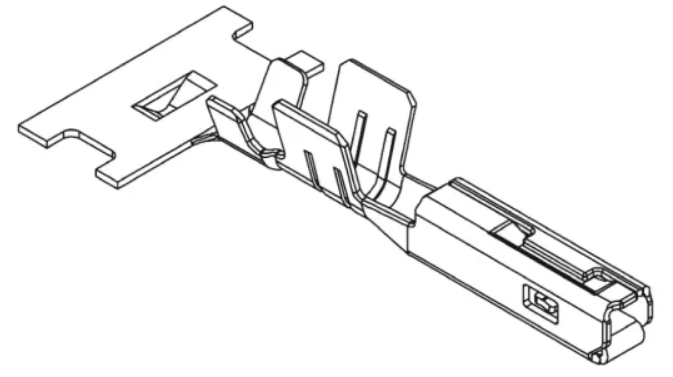
\includegraphics[width=\textwidth]{lisovacka1.png}
  \end{minipage}
  \hfil
  \begin{minipage}[t]{0.32\textwidth}
    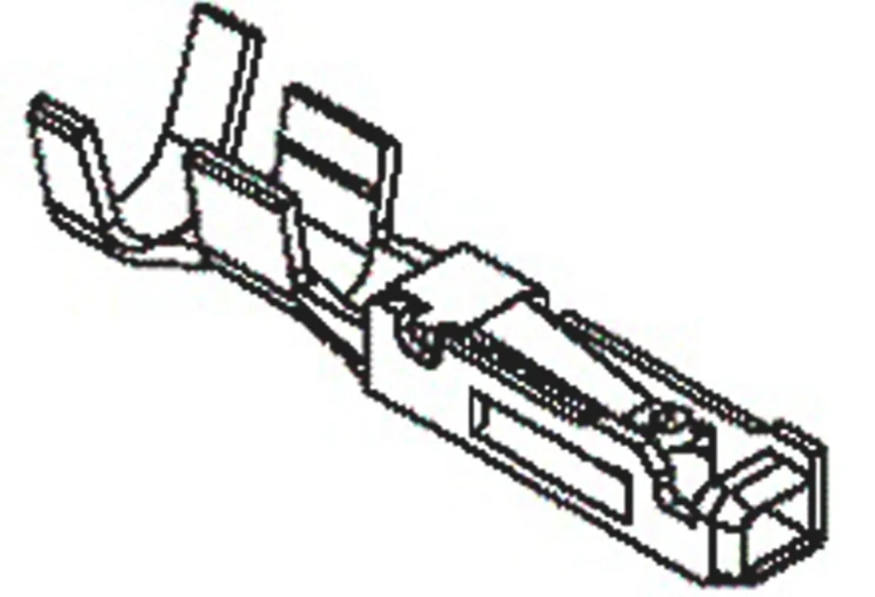
\includegraphics[width=\textwidth]{lisovacka2.png}
    \centering
  \end{minipage}
  \hfil
  \begin{minipage}[t]{0.32\textwidth}
    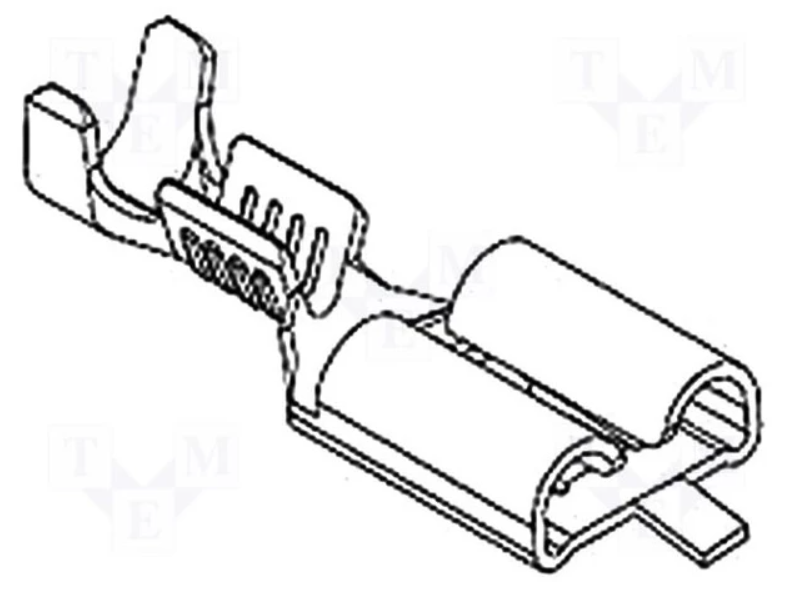
\includegraphics[width=\textwidth]{lisovacka3.png}
    \centering
  \end{minipage}
  \caption{Lisovací kontakty}
\end{figure}

\newpage
\subsection{Press fit konektor}
\begin{itemize}
  \item Připojení vodičů k DPS bez pájení
  \item Nevýhody
  \begin{itemize}
    \item Speciální návrh DPS
  \end{itemize}
\end{itemize}

\begin{figure}[H]
  \begin{minipage}[t]{0.456\textwidth}
    \centering
    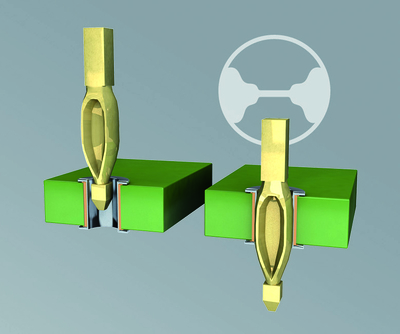
\includegraphics[width=\textwidth]{pressFit1.jpg}
  \end{minipage}
  \hfil
  \begin{minipage}[t]{0.5439\textwidth}
    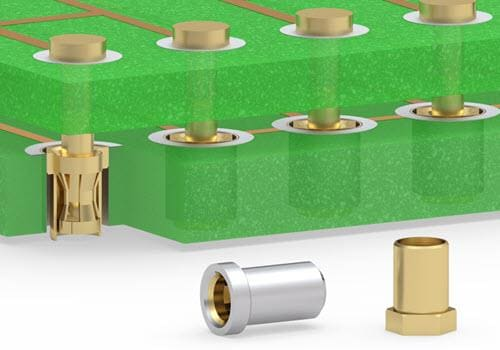
\includegraphics[width=\textwidth]{pressFit2.jpg}
    \centering
  \end{minipage}
  \caption{Lisovací kontakty}
\end{figure}

\section{Připojování vodičů bez odizolování}
Typicky pro ploché vodiče

\begin{figure}[H]
  \begin{minipage}[t]{0.6\textwidth}
    \centering
    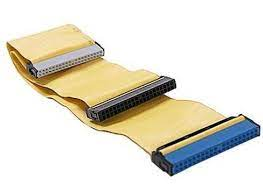
\includegraphics[width=\textwidth]{plochac1.jpg}
  \end{minipage}
  \hfil
  \begin{minipage}[t]{0.4\textwidth}
    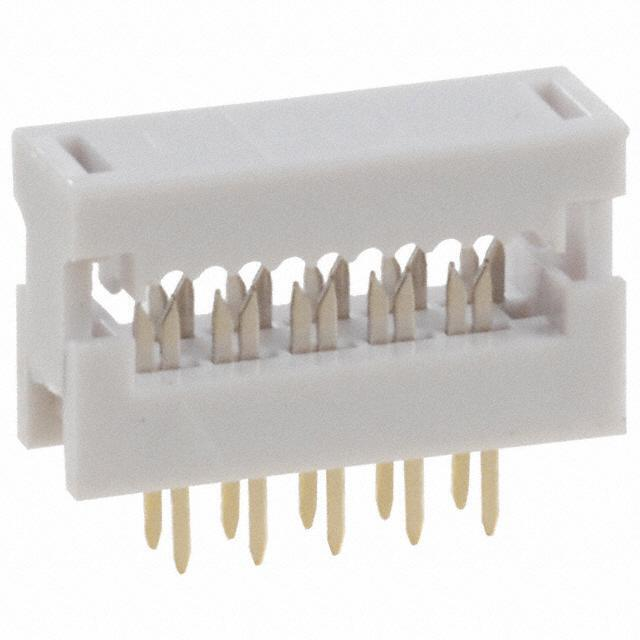
\includegraphics[width=\textwidth]{plochac2.jpg}
    \centering
  \end{minipage}
  \caption{Ploché kabely}
\end{figure}

\end{document}